\section{半导体器件}
P3N5(3p)(穴电),PN结多子扩散形成电流,
\subsection{二极管}
\begin{figure}[H]
    \centering
    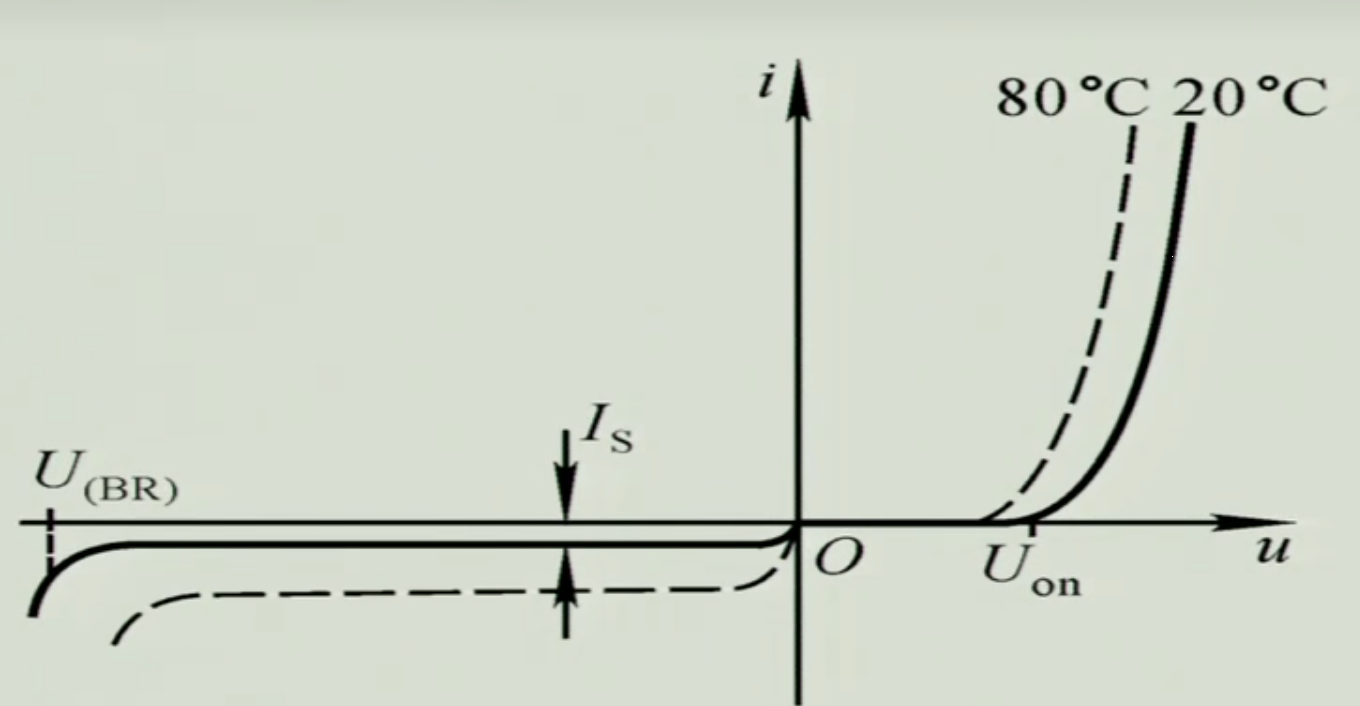
\includegraphics[width=7cm]{./img/1.2.png}
\end{figure}
击穿电压:$U_{BR}$,开启电压:$U_{on}$,反向电流:$I_s$,最高频率$f_m$。温度升高,左下。
\subsubsection{等效电路}
我们需要知道等效电路是什么样子的,用非线性用线性表示出来。有两种,一种是外特性的等效,一种是模型原理上的等效。伏安特性折线化
\begin{theorem}[二极管电流方程]
\[
i=I_s(e^{\frac{u}{U_T}}-1)
\]
\end{theorem}

可以等效成理想,考虑压降,考虑压降和线性斜率,微变等效电路。

对于微变等效电路,已正向导通,有
\begin{equation}
I=I_se^{\frac{U}{U_T}}    \tag{2.1}
\end{equation}
\subsubsection{怎么计算工作状态}
\begin{description}[leftmargin=1.7cm,style=nextline,nosep]% nosep没有垂直间隔
    \item[只有一个] 断开算两端电压
    \item[两个或者多个] 共阴阳只有一个可以正常工作,可以看谁不共的大或者使用\underline{\textbf{假设}}法。
    \item[稳压二极管] 工作在击穿区?
    \item[其他] SI 0.7, GE 0.2    
\end{description}
\subsection{双极型晶体管}
\subsubsection{晶体管的主要参数}
极限参数有最大允许功耗,集电极最大允许电流$I_CM$,反向击穿电压$U_{(BR)CEO}$
% \subsubsection{三极管的h参数等效电路}
% 在交流通路中可将晶体管看成为一个二端口网络,输入回路、输出回路各为一个端口

\subsection{单极型晶体管FET}
低功耗,噪声小,体积小,抗辐照性强,只有\textbf{\underline{多子}}参与导电,\underline{\textbf{压控}}。
分为\underline{结}型(JET)和\underline{绝缘栅}型(MOS管)。
\subsubsection{N沟道增强型绝缘栅型MOS管}
        \begin{figure}[H]
            \centering
            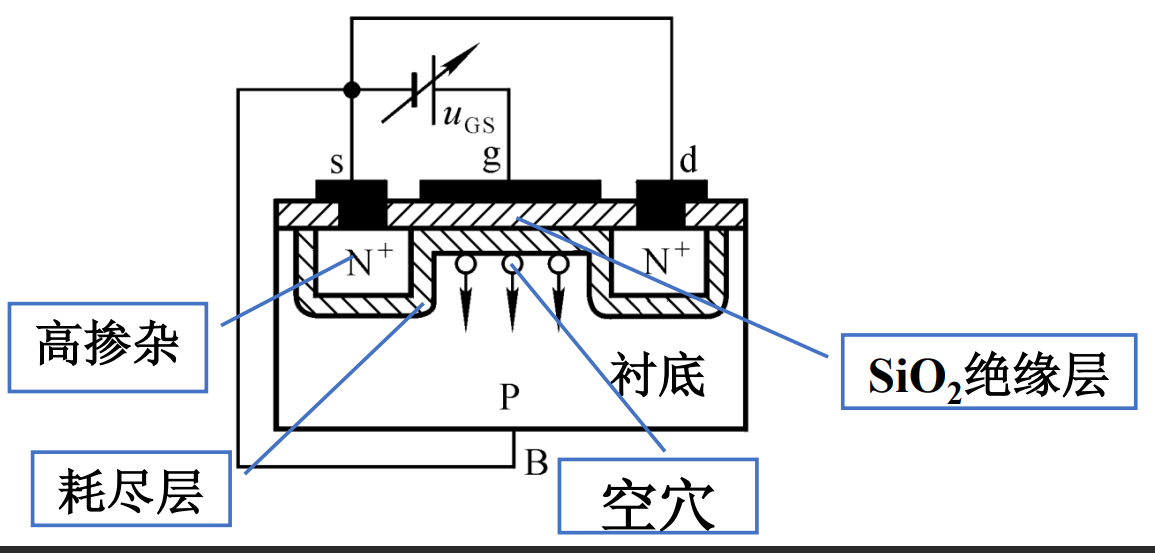
\includegraphics[width=7cm]{img/1.3.png}
            \end{figure}
g 栅极,S 源极,d漏极,分别对应三极管的(b,e,c),$U_{GS}$ 增大到一定程度,再继续增大,
导电沟道将变厚,ds之间\underline{\textbf{电阻}}变小。
        \begin{figure}[H]
            \centering
            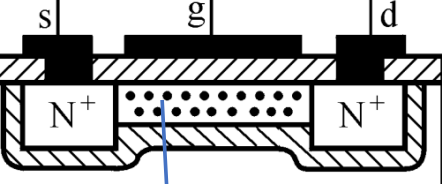
\includegraphics[width=5cm]{img/1.4.png}
            \end{figure}
此时如果要出现电流,那我们只需要在ds两端加一个电压$U_{ds}$就行,此时固定USG,研究$U_{ds}$对$i_D$的影响,gs电位差变小,沟道开始
倾斜,$U_{ds}$增大,沟道越来越倾斜,$i_D$增大,但是增大的速度越来越慢,最后趋于饱和。
        \begin{figure}[H]
            \centering
            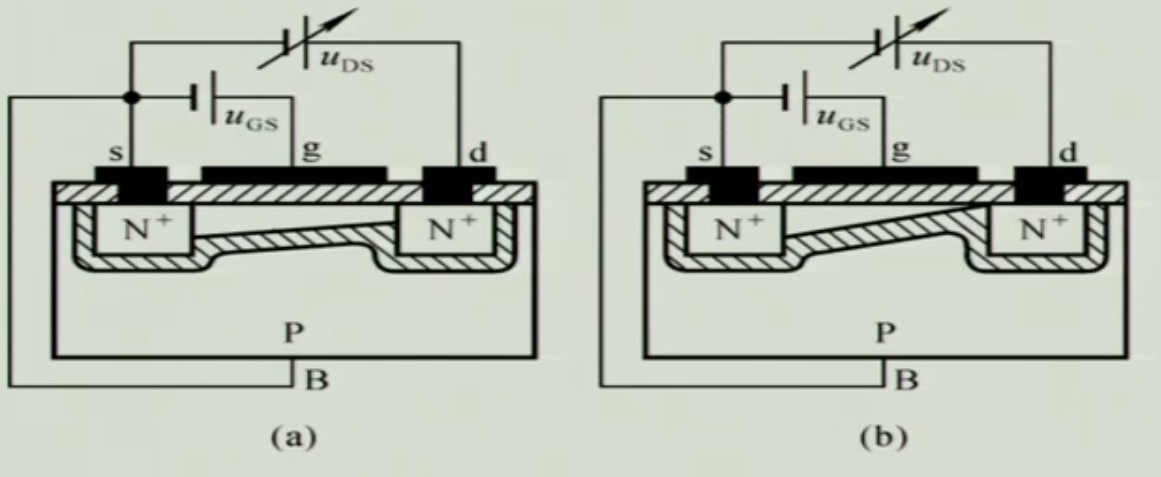
\includegraphics[width=7cm]{img/1.5.png}
            \end{figure}
当$\displaystyle U_{GS}-U_{DS}=U_{GS(th)}$ 成为预夹断,再增加电阻增大,之后近似恒流。
\begin{figure}[H]
    \centering
    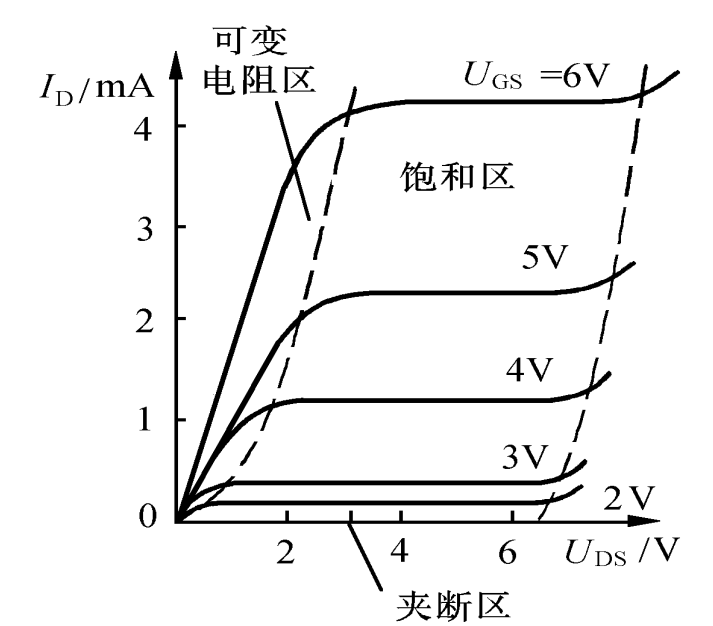
\includegraphics[width=7cm]{img/1.6.png}
    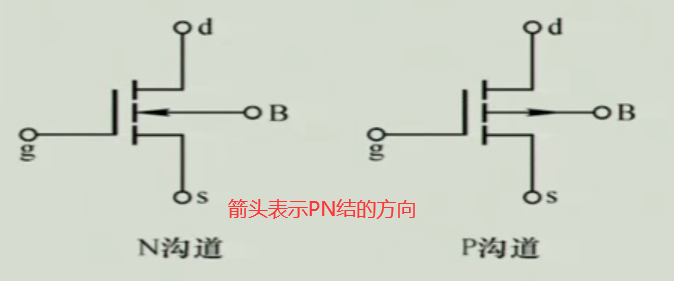
\includegraphics[width=7cm]{img/1.7.png}
    \end{figure}
他本身没有沟道,那能不能让他一开始就有沟道?
\begin{quote}
{\qquad\parindent2\ccwd\kaishu\zihao{5}
N 沟道耗尽型MOS管
}
\subsubsection{N沟道耗尽型绝缘栅型MOS管}
天生有沟道,有一个参数叫做$U_{GS(off)}$,称作夹断电压。
\end{quote}
\subsubsection{N沟道结型场效应管}
        \begin{figure}[H]
            \centering
            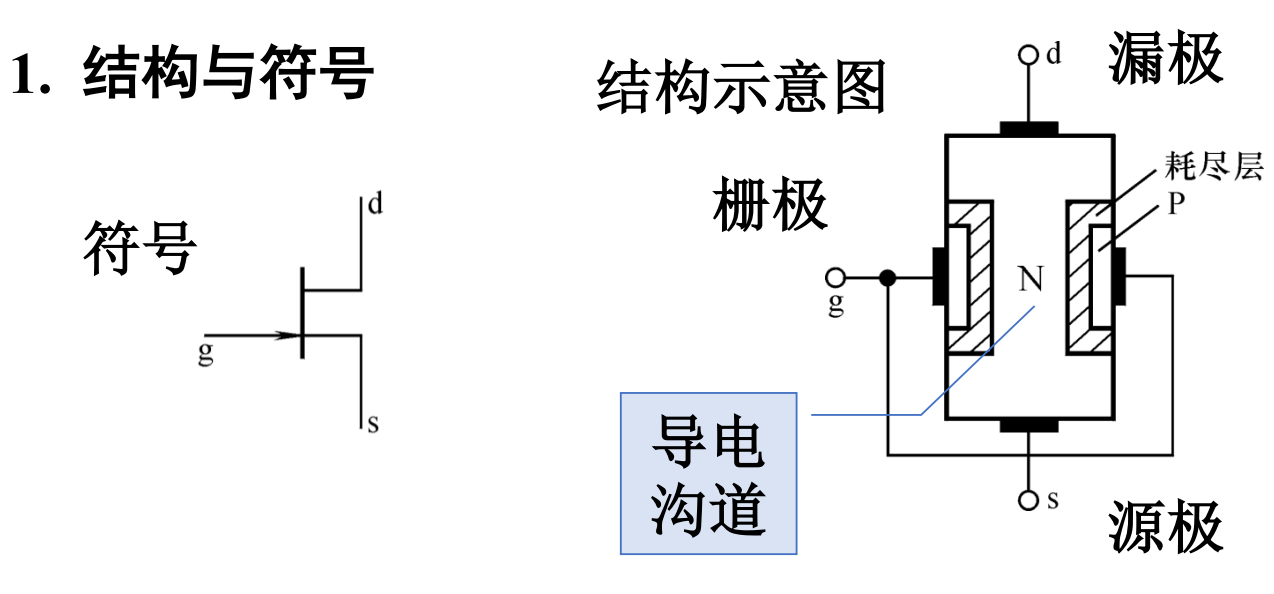
\includegraphics[width=7cm]{img/1.8.png}
            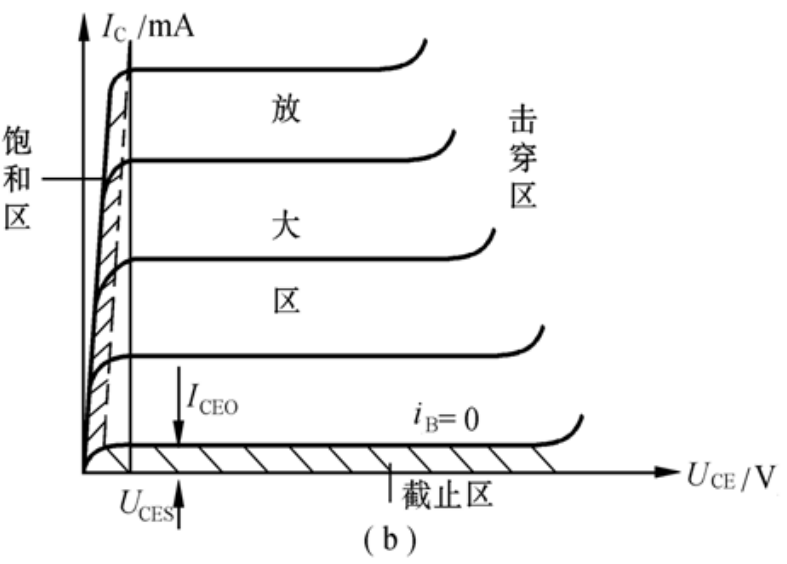
\includegraphics[width=7cm]{img/1.9.png}

            \end{figure}
天生有沟道,加反压使其夹断,是真夹断。

\subsection{场效应管的特性曲线和参数}
漏极,源极和栅极。有转移和输出特性曲线。
\begin{figure}[H]
    \centering
    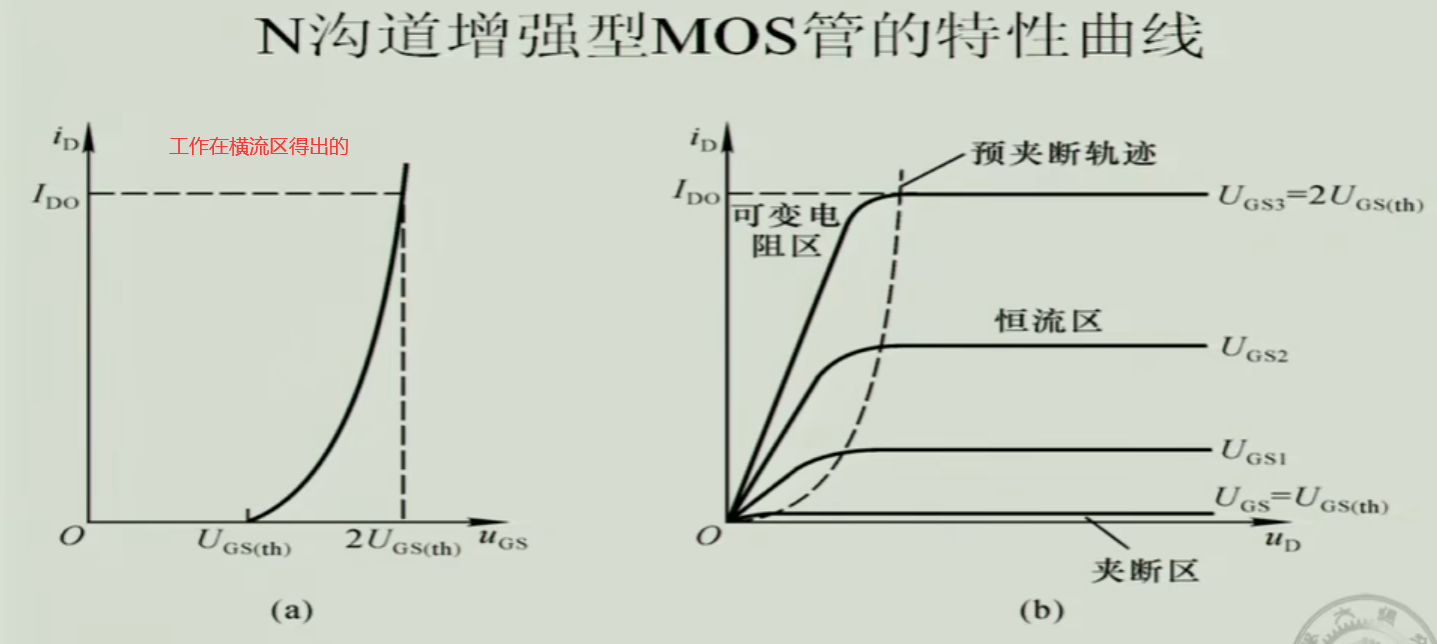
\includegraphics[width=7cm]{img/1.9.1.png}
    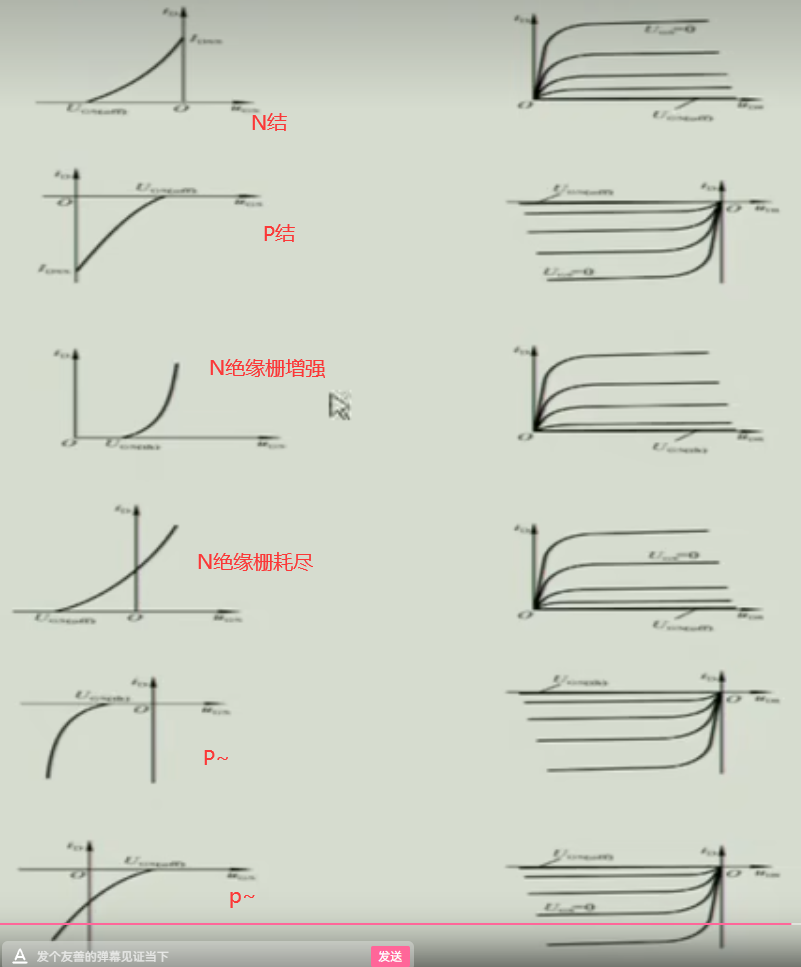
\includegraphics[width=8cm]{img/1.9.2.png}

    \end{figure}
其中漏极电流和gs之间电流方程为(对应上图曲线)
\begin{align}
    i_{D}=I_{DO}(\frac{u_{GS}}{U_{GS(th)}}-1)^{2} \tag{2.1.a} \\
    i_{D}=I_{DSS}(1-\frac{u_{GS}}{U_{GS(off)}})^{2} \tag{2.1.b}
\end{align}

其中$I_{Dss}$为$U_{GS}=0$ 时的漏极电流,
其中$I_{Do}$为$U_{GS}=2U_{GS(th)}$ 时的漏极电流.(2.1.a)是对N沟道绝缘栅型增强(MOS)管,(2.1.b)是对N沟道结型(JET)管。
{直流参数}
$$
U_{GS(th)},U_{GS(off)},I_{Dss},R_{GS(DC)}
$$
{交流参数}
跨导$g_m$